%%% Local Variables: 
%%% mode: latex
%%% TeX-master: "tex_source/main"
%%% End: 
%%% introduction.tex --- 

%% Author: garamonfok@gros
%% Version: $Id: introduction.tex,v 0.0 2011/10/09 18:39:32 garamonfok Exp$

\section{Introduction}

\section{Material and Methods}

\subsection{Dataset}

\subsubsection{Five mammals}

Complete genomes of 5 mammals species (\textit{Homo sapiens}, \textit{Pan troglodytes}, \textit{Mus musculus}, \textit{Rattus norvegicus} and \textit{Canis familiaris}) where retrieved from \textit{Ensembl} \cite{Flicek2011}. Also orthology prediction between each pair of species
possibly done between human and the others was retrieved from \textit{Ensembl Compara} \cite{Vilella2009} using biomart \cite{Kinsella2011}. Only groups of orthologs \textit{one-to-one} with one representative of each species where kept in the final dataset. \ref{fig:phylogeny}
NUMBERS

\subsubsection{6 Drosophila}

\subsection{Alignments}
Each of the group of orthologous sequences were aligned with Muscle \cite{Edgar2004}, and, once aligned sequences were cleaned with trimal \cite{Capella-Gutierrez2009} keeping all sequences but trimming aligment columns with the euristic1 method.


\begin{figure}[htpb] 
\centering 
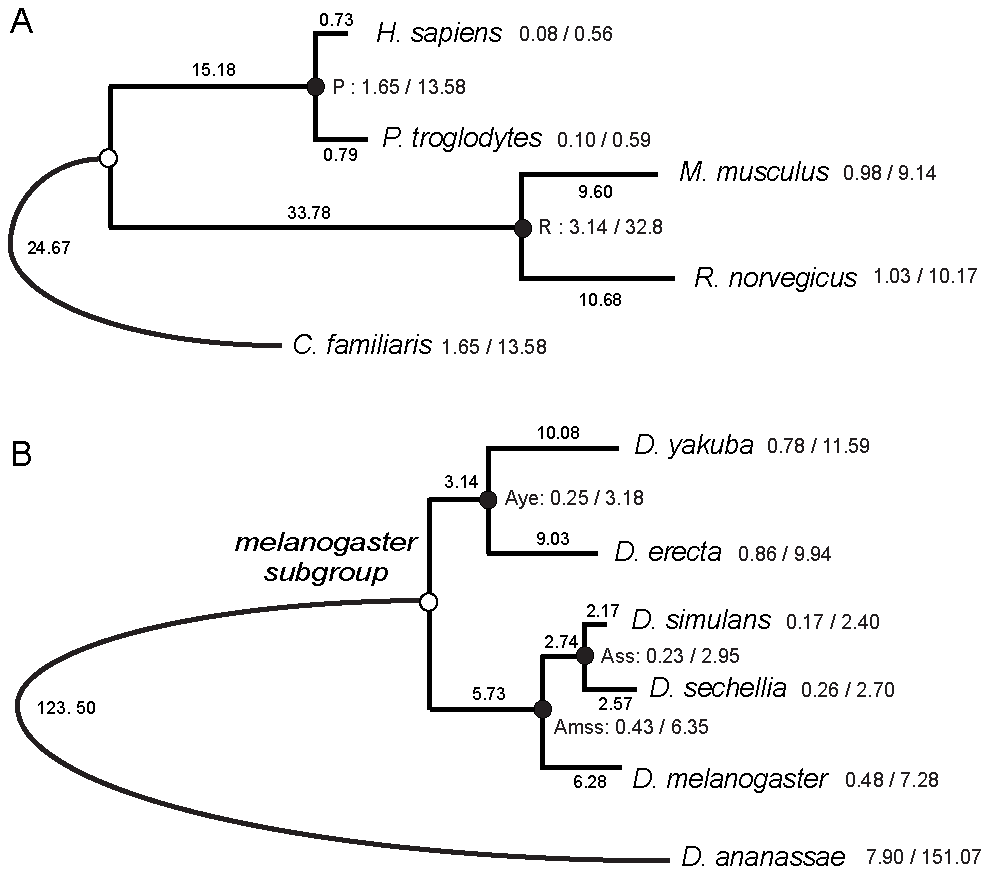
\includegraphics[width=\textwidth]{tex_source/figures/gssa/phylogenies.png}
\caption[Mammals and \textit{Drosophila} phylogeny]{Mammals and
  \textit{Drosophila} phylogeny. blabli blob lu dkfnlskjdf}
\label{fig:phylogeny}
\end{figure}


\section{open on colocalization to not random}

